\section{Affine transforms}

The act of altering the coordinates of an object's points is termed a transformation. 
In three-dimensional space, transformations can be intricate, potentially relocating all points of the object.
Nevertheless, a significant and extensive array of transformations can be encapsulated using a mathematical concept known as affine transforms.

Objects in 3D space are delineated by the coordinates of their points. 
Through the application of affine transformations to these point coordinates, objects can be translated, rotated, or scaled within the 3D space.

Affine transforms are typically categorized into four classes: translation, scaling, rotation, and shear. 
When translating, rotating, or scaling an object, the identical transformation is applied to all its points. 
The resultant transformed object is derived by reconstructing the geometric primitive using the updated points.

\paragraph*{Matrix transforms}
In the realm of homogeneous coordinates, $4 \times 4$ matrices serve as the tool to express various geometrical transformations. 
The transformed vertex $p^\prime$ is obtained from the original point $p$ by a straightforward matrix multiplication with the corresponding transformation matrix $M$:
\[p^\prime = M \cdot p^T = \left( x^\prime, y^\prime, z^\prime, 1 \right)\]
It's worth noting that there are two conventions in use:
\begin{itemize}
    \item The transformation matrix $M$ appears on the left side of the multiplication.
    \item The transformation matrix $M$ appears on the right side.
\end{itemize}
For consistency, we adopt the convention where the matrix appears on the left.

\subsection{Identity transform}
The identity transformation leaves the points of an object unchanged. 
It is represented by a $4 \times 4$ identity matrix:
\[M=I=\begin{bmatrix}
    1 & 0 & 0 & 0 \\
    0 & 1 & 0 & 0 \\
    0 & 0 & 1 & 0 \\
    0 & 0 & 0 & 1 \\
\end{bmatrix}\]

\begin{figure}[H]
    \centering
    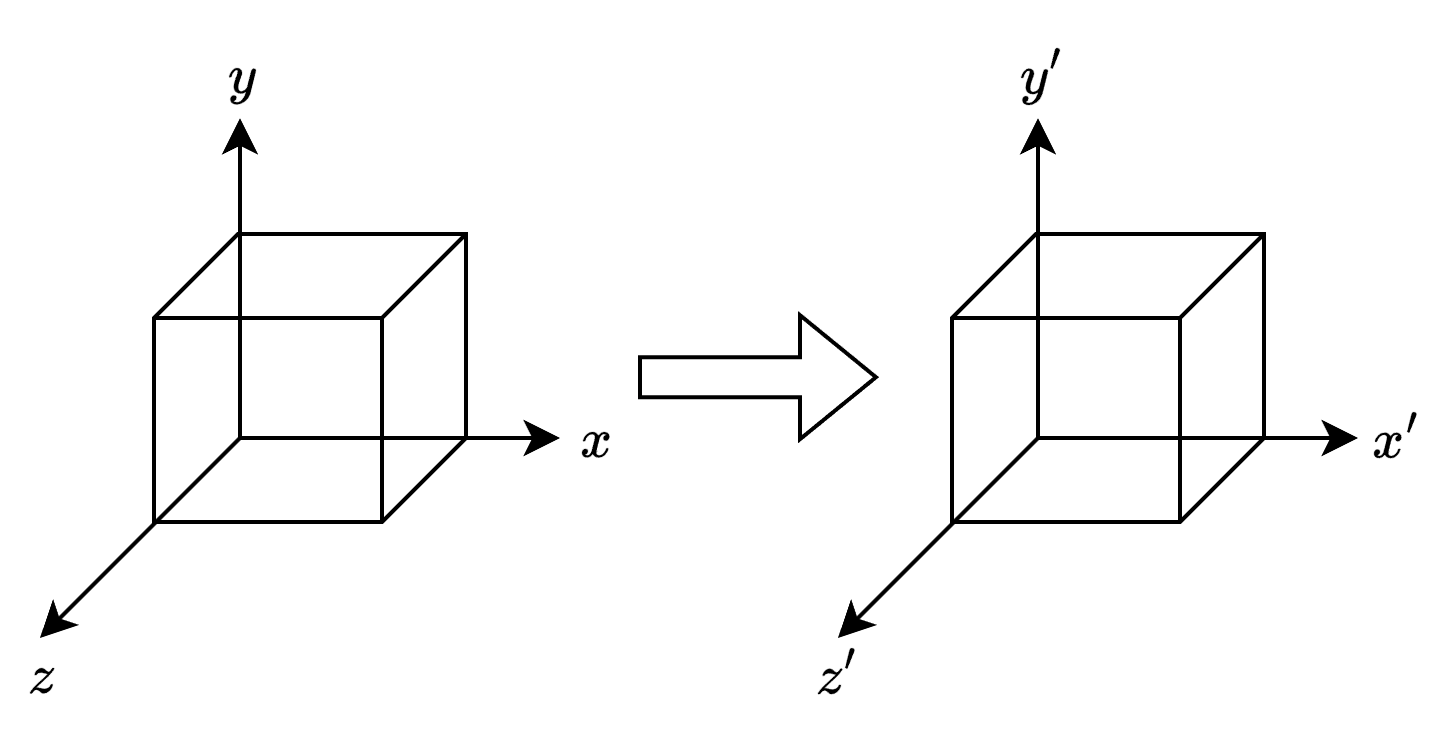
\includegraphics[width=0.65\linewidth]{images/identity.png}
    \caption{Identity transform}
\end{figure}

\subsection{Translation}
To move an object by distances $d_x$, $d_y$, and $d_z$ along the $x$-axis, $y$-axis, and $z$-axis respectively, the new coordinates can be obtained by simply adding these distances to each corresponding axis:
\[\begin{cases}
    x^\prime=x+d_x \\ 
    y^\prime=y+d_y \\ 
    z^\prime=z+d_z 
\end{cases}\]
In homogeneous coordinates derived from Cartesian coordinates, where the fourth component is always $w=1$, the translation matrix $T(d_x, d_y, d_z)$ can be constructed by placing $d_x$, $d_y$, and $d_z$ in the last column of the identity matrix:
\[M=T(d_x , d_y , d_z)=\begin{bmatrix}
    1 & 0 & 0 & d_x \\
    0 & 1 & 0 & d_y \\
    0 & 0 & 1 & d_z \\
    0 & 0 & 0 & 1   \\
\end{bmatrix}\]

\begin{figure}[H]
    \centering
    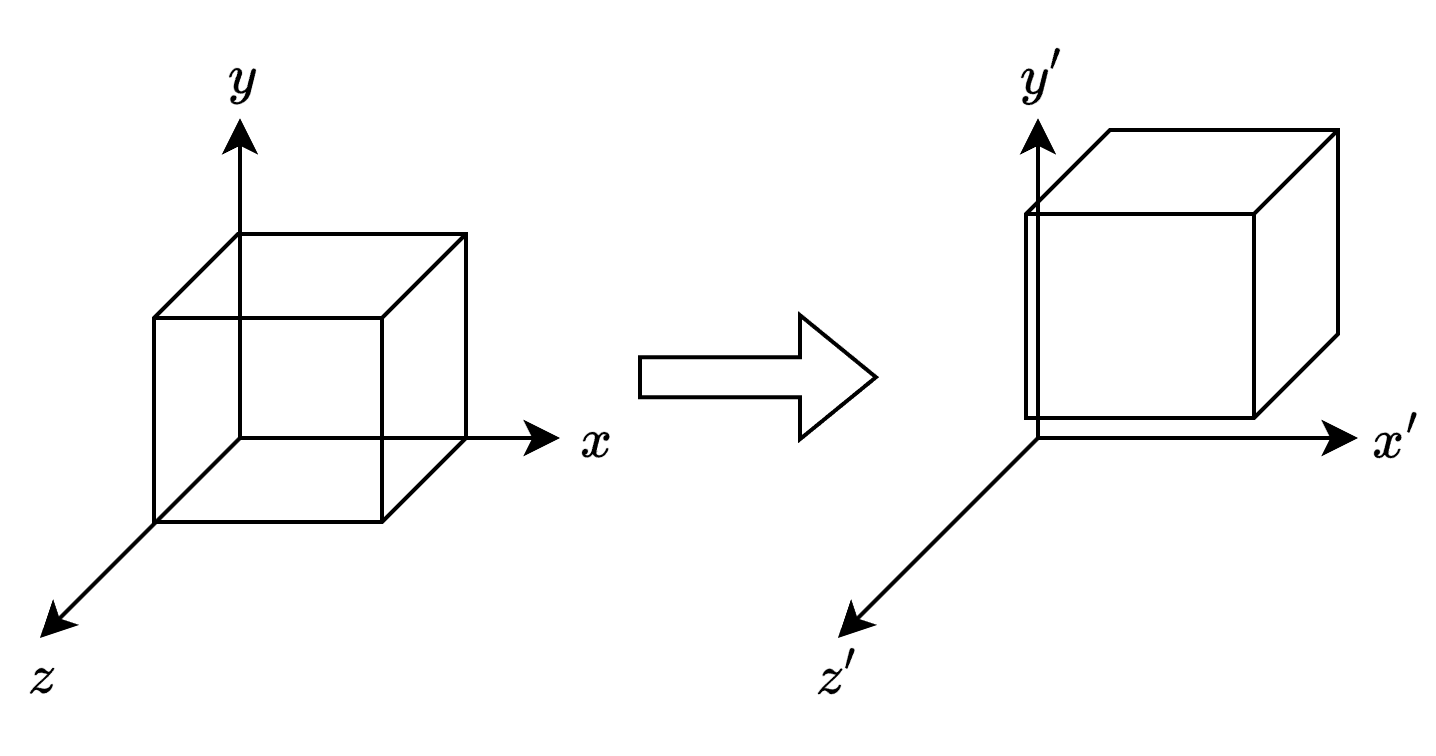
\includegraphics[width=0.65\linewidth]{images/traslation.png}
    \caption{Translation transform}
\end{figure}

\subsection{Scaling}
Scaling alters the size of an object while preserving its position and orientation. 
It can be employed for various effects such as enlargement, shrinkage, deformation, mirroring, and flattening. 
Scaling transformations are characterized by a center, a fixed point that remains unchanged during the transformation. 
Initially, we assume the scaling center is at the origin of the 3D space.

Proportional scaling uniformly magnifies or diminishes an object by the same factor $s$ in all directions. 
Consequently, it preserves the object's proportions while changing its size. 
The coordinates of points are modified by multiplying each coordinate by the scaling factor $s$:
\[\begin{cases}
    x^\prime=s \cdot x \\ 
    y^\prime=s \cdot y \\ 
    z^\prime=s \cdot z 
\end{cases}\]
Depending on the value of $s$, the transformation can either enlarge (for $s > 1$) or shrink (for $0 < s < 1$) the object.
Non-proportional scaling distorts an object using different scaling factors $s_x$, $s_y$ and $s_z$ for each axis, allowing enlargement or shrinkage in only one direction.
Initially, non-proportional scaling is considered along the three main axes. 
The new coordinates are computed as:
\[\begin{cases}
    x^\prime=s_x \cdot x \\ 
    y^\prime=s_y \cdot y \\ 
    z^\prime=s_z \cdot z 
\end{cases}\]
The scaling transformation matrix $S(s_x , s_y , s_z)$ is formed by placing the scaling factors $s_x$, $s_y$ and $s_z$ on the diagonal:
\[M=S(s_x , s_y , s_z)=\begin{bmatrix}
    s_x & 0   & 0   & 0 \\
    0   & s_y & 0   & 0 \\
    0   & 0   & s_z & 0 \\
    0   & 0   & 0   & 1 \\
\end{bmatrix}\]
It's worth noting that proportional scaling is a special case achieved when using identical scaling factors $s=s_x=s_y=s_z$. 

\begin{figure}[H]
    \centering
    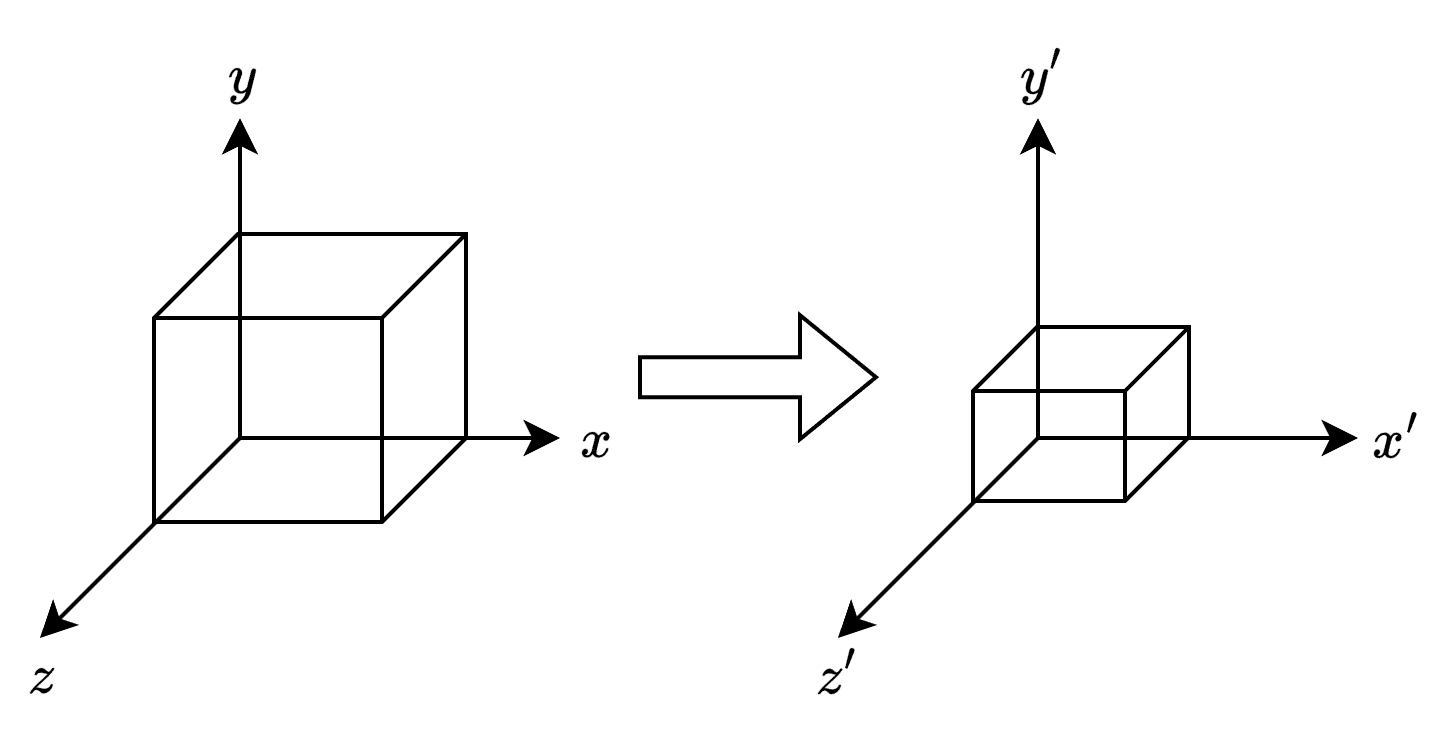
\includegraphics[width=0.65\linewidth]{images/scaling.png}
    \caption{Scaling transform}
\end{figure}

\paragraph*{Mirroring}
Mirroring can be achieved by utilizing negative scaling factors.
Initially, we assume the mirror occurs around a plane or axis passing through the origin, aligned with the $x$, $y$ or $z$ axes.
Three types of mirroring are possible:
\begin{itemize}
    \item \textit{Planar}: this creates a symmetric object with respect to a plane. 
        It's accomplished by setting -1 as the scaling factor for the axis perpendicular to the plane ($x$ for $yz$-plane): 
        \[\begin{cases}
            s_x = -1 \\ 
            s_y = 1  \\ 
            s_z = 1 
        \end{cases}\]
    \item \textit{Axial}: this creates a symmetric object with respect to an axis. 
        It's achieved by setting -1 as the scaling factor for all axes except the one corresponding to the axis of symmetry ($x$ and $z$ for the $y$-axis): 
        \[\begin{cases}
            s_x = -1 \\ 
            s_y = 1  \\ 
            s_z = -1 
        \end{cases}\]
    \item \textit{Central}: this creates a symmetric object with respect to the origin. 
        It's accomplished by setting -1 as the scaling factor for all axes:
        \[\begin{cases}
            s_x = -1 \\ 
            s_y = -1 \\ 
            s_z = -1 
        \end{cases}\]
\end{itemize}

\paragraph*{Flattening}
When a scaling factor of 0 is applied in any direction, it flattens the image along that axis. 
However, this operation must be approached with caution as it effectively reduces the dimensionality of the objects.
For the sake of simplicity in our discussion, we will typically assume that the scaling coefficients are non-zero.

\subsection{Rotation}
Rotation alters the orientation of an object while keeping its position and size unchanged.
It is performed along an axis, a line where points remain unaffected by the transformation.
Initially, we will focus on rotations about the three reference axes passing through the origin.

A rotation of an angle $\alpha$ about the $z$-axis can be computed as follows:
\[\begin{cases}
    x^\prime = x \cdot \cos \alpha - y \cdot \sin \alpha \\
    y^\prime = x \cdot \sin \alpha - y \cdot \cos \alpha \\
    z^\prime = z
\end{cases}\]
Expressed in matrix form, this becomes:
\[R_x(\alpha)=
\begin{bmatrix}
    1 & 0   & 0   & 0 \\
    0   & \cos \alpha & - \sin \alpha   & 0 \\
    0   & \sin \alpha   & \cos \alpha & 0 \\
    0   & 0   & 0   & 1 \\
\end{bmatrix}\]
Utilizing homogeneous coordinates, rotations of an angle $\alpha$ around the $z$-axis can be represented by matrices.
Rotations about the $x$-axis and the $y$-axis follow similar principles and are expressed by the following matrices:
\[R_y(\alpha)=
\begin{bmatrix}
    \cos \alpha & 0   & \sin \alpha   & 0 \\
    0   & 1 & 0 & 0 \\
    -\sin \alpha  & 0   & \cos \alpha & 0 \\
    0   & 0   & 0   & 1 \\
\end{bmatrix} 
\qquad 
R_z(\alpha)=
\begin{bmatrix}
    \cos \alpha & -\sin \alpha  & 0   & 0 \\
    \sin \alpha   & \cos \alpha & 0 & 0 \\
    0  & 0   & 1 & 0 \\
    0   & 0   & 0   & 1 \\
\end{bmatrix}\]

\begin{figure}[H]
    \centering
    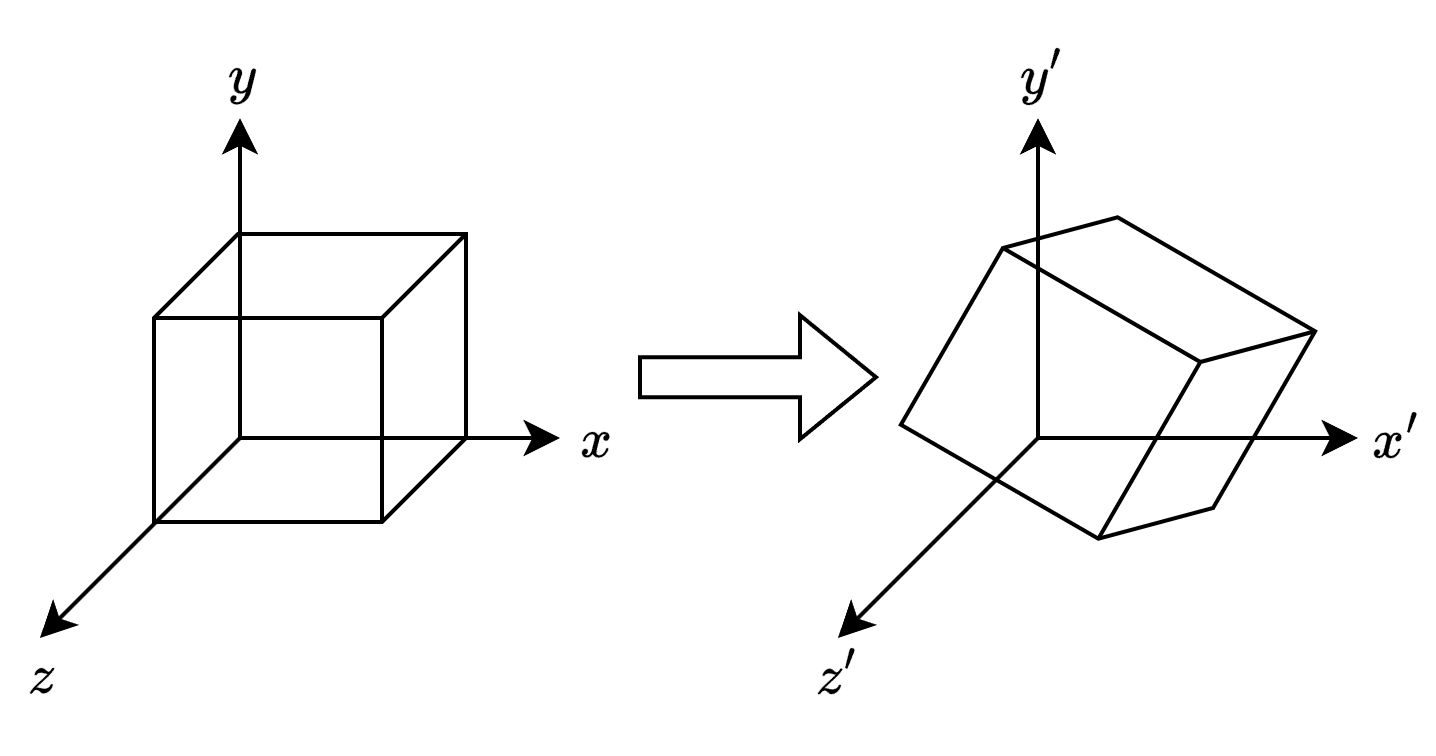
\includegraphics[width=0.64\linewidth]{images/rotation.png}
    \caption{Rotation transform}
\end{figure}

\subsection{Shear}
The shear transform bends an object in one direction and is performed along an axis with a center. 
Initially, we focus on the $y$-axis passing through the origin.
As the value of the $y$-axis increases, the object is linearly bent into a direction specified by a 2D vector (defined by $h_x$ and $h_z$).
The transformed point coordinates are computed as follows:
\[\begin{cases}
    x^\prime = x + y \cdot h_x \\
    y^\prime = y \\
    z^\prime = z + y \cdot h_z
\end{cases}\]
In matrix form, this becomes:
\[H_x(h_y,h_z)=
\begin{bmatrix}
    1   & 0   & 0   & 0 \\
    h_y   & 1   & 0   & 0 \\
    h_z   & 0   & 1   & 0 \\
    0   & 0   & 0   & 1 \\
\end{bmatrix}\]
Similarly, shear transforms can be applied along the $x$-axis and the $z$-axis:
\[H_y(h_x,h_z)=
\begin{bmatrix}
    1   & h_x   & 0   & 0 \\
    0   & 1   & 0   & 0 \\
    0   & h_z   & 1   & 0 \\
    0   & 0   & 0   & 1 \\
\end{bmatrix}
\qquad 
H_z(h_x,h_y)=
\begin{bmatrix}
    1   & 0   & h_x   & 0 \\
    0   & 1   & h_y   & 0 \\
    0   & 0   & 1   & 0 \\
    0   & 0   & 0   & 1 \\
\end{bmatrix}\]

\begin{figure}[H]
    \centering
    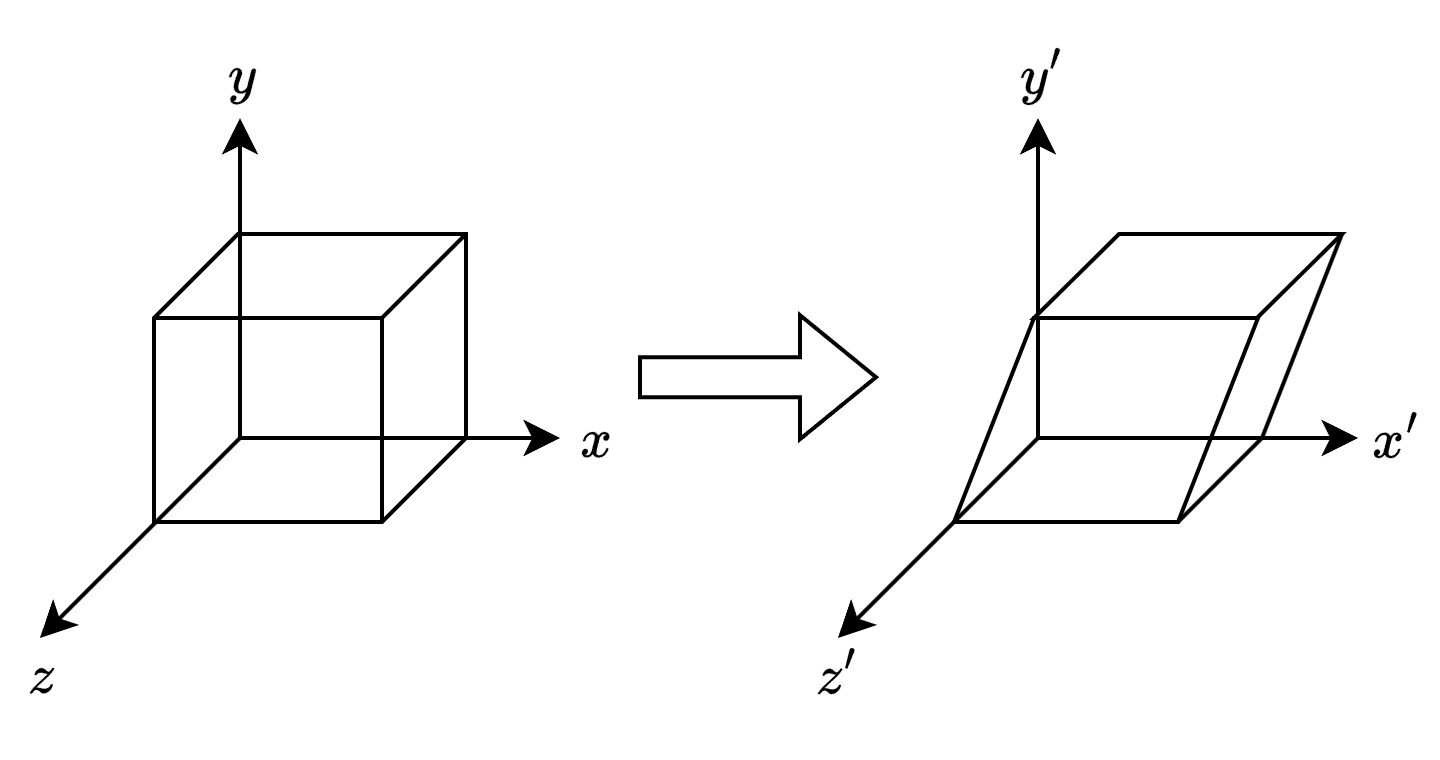
\includegraphics[width=0.65\linewidth]{images/shear.png}
    \caption{Shear transform}
\end{figure}

\subsection{Transformation matrix}
It's important to note that in all the $4 \times 4$ transformation matrices we've discussed, the last row is always $\begin{bmatrix} 0 & 0 & 0 & 1\end{bmatrix}$. 
This ensures that the $w$ coordinate remains unchanged by the transformation.

The upper part of a transformation matrix can be split into a $3\times 3$ sub-matrix $M_R$, representing the rotation, scaling, and shear factors of the transform, and a column vector $d^T$ encoding the translation:
\[M=
\begin{bmatrix}
    n_{xx} & n_{yx} & n_{zx} & d_x \\ 
    n_{xy} & n_{yy} & n_{zy} & d_y \\
    n_{xz} & n_{yz} & n_{zz} & d_z \\
    0      & 0      & 0      & 1   \\
\end{bmatrix}= 
\begin{bmatrix}
    M_R & d^T \\ 
    0 & 1
\end{bmatrix}
\]
Specifically, the matrix product exchanges the three Cartesian axes of the original coordinate system with three new directions. 
The columns of $M_R$ represent the directions and sizes of the new axes in the old reference system.
\begin{figure}[H]
    \centering
    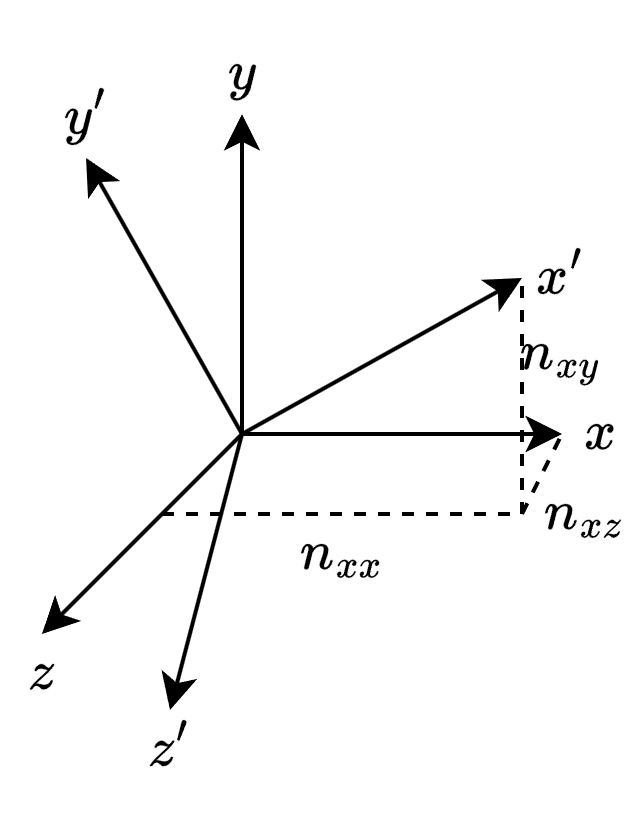
\includegraphics[width=0.3\linewidth]{images/mr.png}
    \caption{Transformation matrix $M_R$}
\end{figure}
The vector $d^T$ represents the position of the origin of the new coordinate system in the old one.
\begin{figure}[H]
    \centering
    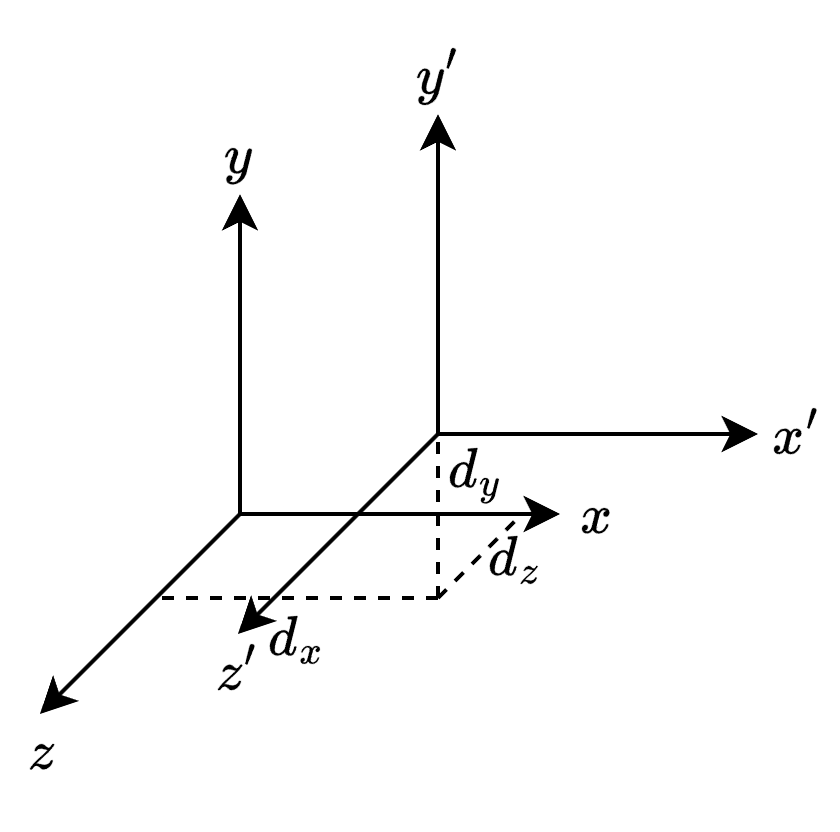
\includegraphics[width=0.35\linewidth]{images/dt.png}
    \caption{Transformation matrix $d_t$}
\end{figure}
The transformation introduces the following changes to the axes:
\begin{itemize}
    \item Rotations maintain the size and angles of the axes constant but change their directions.
    \item Scaling increases or decreases the size of the axes while maintaining their original directions.
    \item Shear bends the axes along which the transform is performed.
\end{itemize}
In many cases, it's simpler to define a transformation by specifying its new center and the new directions of its axes.

\paragraph*{Conventions}
It's important to highlight that under the matrix-on-the-right convention, all transformation matrices are transposed.
A simple way to identify which convention is being used is by inspecting a non-zero translation transform:
\begin{itemize}
    \item If the matrix has the last column $\begin{bmatrix}0 & 0 & 0 & 1\end{bmatrix}$, then the matrix-on-the-right convention is employed.
    \item Conversely, if the last row is $\begin{bmatrix}0 & 0 & 0 & 1\end{bmatrix}$, then the matrix-on-the-left convention is being utilized.
\end{itemize}